% ------------------------------------------------------------------------
% file `math2-exercise-67-exercise-body.tex'
%   in folder `xsim/'
%
%     exercise of type `exercise' with id `67'
%
% generated by the `exercise' environment of the
%   `xsim' package v0.11 (2018/02/12)
% from source `math2' on 2021/07/22 on line 420
% ------------------------------------------------------------------------
À partir de la figure ci-dessous, complète les égalités, en sachant que $M$ représente le milieu de $\lbrack BC \rbrack$.
    \begin{center}
        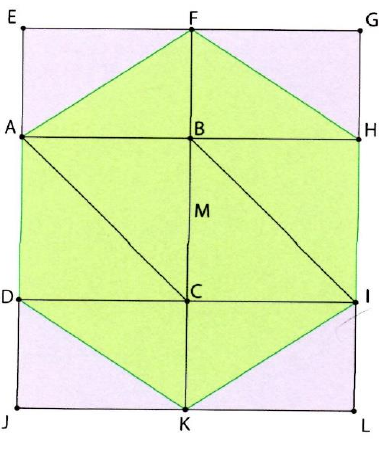
\includegraphics[width=.5\linewidth]{transformation-du-plan/img/ex03.png}
    \end{center}
    \begin{tasks}
        \task $S_{M}(ABC)=\dotfill$
        \task $S_{AC}(B) = \dotfill$
        \task $t_{\overrightarrow{EF}}(\left\lbrack JK) \right\rbrack = \dotfill$
        \task $S_{BK}(G) = \dotfill $
        \task $t_{\overrightarrow{HB}}\dotfillbox[3cm] =  ABC$
        \task $S_{\dotfillbox}(C) = H$
        \task $S_{FB}\dotfillbox[2cm]=  HGF$
        \task $S_{M}(\left\lbrack EG \right\rbrack) = \dotfill $
    \end{tasks}
